\title{\textbf{AEGIS-V5: Adaptive Enhanced Global-Local Integrated Sparse Attention with SVD-Factorized Projections}}

\author{Anonymous authors}


\section{Introduction}

\subsection{Motivation}

Transformer self-attention scales quadratically with sequence length $L$, 
in both compute and memory. For input $X \in \mathbb{R}^{B \times L \times d}$ 
with $H$ heads, the intermediate attention matrix $Q K^\top \in \mathbb{R}^{L \times L}$ 
costs $\mathcal{O}(L^2)$ per batch item. At $L = 4096$, this is ~16M 
entries per head, becoming prohibitive for long-context workloads.

Existing methods address this along three axes:

\begin{enumerate}
\item \textbf{Sparse attention} (Longformer, BigBird) restricts the attention
  pattern to $\mathcal{O}(L \sqrt{L})$ connections.
\item \textbf{Low-rank attention} (Linformer, Nystr mformer) projects $K, V$ to a
  smaller space.
\item \textbf{Kernel attention} (Performer, Linear Transformer) factorizes the
  softmax kernel into feature maps, achieving $\mathcal{O}(L)$.

\end{enumerate}
Each has trade-offs. Sparse methods lose global context; low-rank methods 
require fixed rank; kernel methods suffer from approximation error on 
peaked distributions.

\textbf{Hybrid attention} combines multiple strategies. AEGIS-V5 combines local 
windowed attention (exact, preserves local detail) with global kernel 
linear attention (approximate, captures long-range dependencies).

\subsection{Problem Statement}

Given a pretrained transformer $\mathcal{M}$ with $H$ heads, we seek an 
attention mechanism $\mathcal{A}'$ such that:

\[
\mathcal{A}' \approx \mathcal{A}, \qquad
\text{Cost}(\mathcal{A}') \ll \mathcal{O}(L^2)
\]

subject to:

\begin{enumerate}
\item \textbf{Multi-architecture compatibility:} Must work on DistilBERT (flat),
  RoBERTa (nested), GPT-2 (Conv1D), and Qwen3.5 (GQA + RoPE).
\item \textbf{Causal correctness:} Decoders must preserve causality.
\item \textbf{Parameter efficiency:} Base weights frozen; only LoRA adapters trained.
\item \textbf{Numerical stability:} No NaNs, no silent collapses.

\end{enumerate}
\subsection{Our Approach}

AEGIS-V5 has four key components:

\subsubsection{Split-Head Architecture}

We partition $H$ heads into:

\begin{itemize}
\item $H_\text{local} = \lceil 2H/3 \rceil$ heads using \textbf{local windowed attention}
\item $H_\text{global} = H - H_\text{local}$ heads using \textbf{kernel linear attention}

\end{itemize}
This design lets the model allocate capacity adaptively: most heads focus 
on local structure, a few capture global context.

\subsubsection{Energy-Based SVD Factorization}

Each projection $W$ is decomposed via SVD, and the rank $r$ is chosen to 
capture a target \textbf{energy} fraction:

\[
r^* = \min \left\{ r : \frac{\sum_{i \leq r} \sigma_i^2}{\sum_i \sigma_i^2} \geq \eta \right\}
\]

where $\eta = 0.95$ by default.

\subsubsection{LoRA on Frozen SVD Factors}

The SVD factors $(U_r, V_r)$ are frozen; LoRA adapters provide trainable 
capacity:

\[
\Delta W = \frac{\alpha}{r_L} B A
\]

\subsubsection{Per-Head Adaptive Gating}

The local and global outputs are combined with a learnable per-head gate:

\[
\text{Out} = \sigma(g_h) \cdot \text{Out}_\text{local} + (1 - \sigma(g_h)) \cdot \text{Out}_\text{global}
\]

Gate bias is initialized to $+2.0$, giving $\sigma(2.0) \approx 0.88$ 
(mostly local at start).

\subsection{Contributions}

We make the following contributions:

\begin{itemize}
\item \textbf{A hybrid split-head attention.} AEGIS-V5 combines local windowed and
  global kernel attention, with per-head adaptive gating.
\item \textbf{Energy-based SVD factorization.} Base projections are compressed with
  a target energy fraction, giving explicit control over rank.
\item \textbf{A production-hardened implementation.} Handles four architectures with
  GQA, RoPE, nested encoders, Conv1D, and safe fallback.
\item \textbf{Numerical stability fixes.} We replaced the original ReLU-based \texttt{softpick}
  (which returned all-zeros on masked rows) with a stable softmax-based
  variant, eliminating a subtle collapse mode.
\item \textbf{Full reproducibility.} Code and checkpoints released.

\end{itemize}
\subsection{Paper Organization}

Section 2 reviews related work. Section 3 provides background on attention, 
SVD, LoRA, and kernel methods. Section 4 presents AEGIS-V5. Section 5 
describes integration. Section 6 details the setup. Section 7 reports 
results. Section 8 analyzes trade-offs. Section 9 discusses practical 
guidance. Section 10 lists limitations. Section 11 concludes.



\subsection{Notation}

\begin{lstlisting}

---
\end{lstlisting}

\section{Related Work}

\subsection{Sparse and Local Attention}

\textbf{Longformer} (Beltagy et al., 2020) combines a sliding window with a small 
set of global tokens. \textbf{BigBird} (Zaheer et al., 2020) adds random 
attention and proves Turing completeness. \textbf{Star-Transformer} (Guo et al., 
2019) uses a star topology with a single global hub.

\textbf{Our distinction.} AEGIS-V5 uses exact local attention (not a sparse 
approximation) for the local branch, and a fully-connected kernel 
attention for the global branch.

\subsection{Kernel and Linear Attention}

\textbf{Performer} (Choromanski et al., 2021) uses positive orthogonal random 
features (PORF). \textbf{Linear Transformer} (Katharopoulos et al., 2020) uses 
$\phi(x) = \text{elu}(x) + 1$. \textbf{Random Feature Attention} (Peng et al., 
2021) uses Gaussian RFF.

\textbf{Our distinction.} AEGIS-V5 applies kernel attention **only to a subset 
of heads** (the global heads), preserving exact local computation for the 
rest.

\subsection{Low-Rank Factorization}

\textbf{Linformer} (Wang et al., 2020) projects $K, V$ to a fixed rank. 
\textbf{Nystr mformer} (Xiong et al., 2021) uses Nystr m landmarks. \textbf{ALBERT} 
(Lan et al., 2020) shares parameters across layers.

\textbf{Our distinction.} AEGIS-V5 uses \textbf{energy-based rank selection} for each 
projection independently, and combines SVD with LoRA for recovery.

\subsection{Hybrid Attention}

\textbf{H-Transformer-1D} (Zhu \& Soricut, 2021) uses hierarchical attention. 
\textbf{NHA} (our prior work) combines local sliding window with global linear 
attention via a single scalar gate. \textbf{LEKAv3} (our prior work) uses 
learned landmarks with local window fusion.

\textbf{Our distinction.} AEGIS-V5 uses a \textbf{split-head} architecture: different 
heads use different attention mechanisms. This is more expressive than 
combining branches with a single gate.

\subsection{Parameter-Efficient Fine-Tuning}

\textbf{LoRA} (Hu et al., 2021) freezes base weights and trains low-rank 
adapters. \textbf{AdaLoRA} (Zhang et al., 2023) adaptively allocates rank per 
layer. \textbf{DoRA} (Liu et al., 2024) decomposes weights into magnitude and 
direction.

\textbf{Our distinction.} AEGIS-V5 combines SVD factorization of base weights 
with LoRA adapters on the factorized form, providing both compression and 
recovery.

\subsection{Position of Our Work}

\begin{table*}[t]
\centering
\small
\begin{tabular}{lllllllllll}
\toprule
\textbf{Model} & \textbf{Module} & \textbf{Acc} & \textbf{$\Delta$} & \textbf{Status} & \textbf{F1} & \textbf{Comp.} & \textbf{Ratio} & \textbf{VRAM} & \textbf{Inference (s)} & \textbf{Compression (s)} \\
\midrule
DistilBERT & full & 90.71\% & -- & -- & 0.9099 & 0 & 1.00$\times$ & 183 MB & 1.90 & -- \\
DistilBERT & \textbf{Aegis V5 Module} & \textbf{80.96\%} & -9.98\% & PASS & 0.8379 & 24 & \textbf{0.99$\times$} & 208.3 MB & 25.0 & -- \\
RoBERTa & full & 94.38\% & -- & -- & 0.9445 & 0 & 1.00$\times$ & 293 MB & 4.10 & -- \\
RoBERTa & \textbf{Aegis V5 Module} & \textbf{50.92\%} & +0.00\% & PASS_LOW & 0.6748 & 48 & \textbf{0.94$\times$} & 385.2 MB & 49.1 & -- \\
GPT-2 & full & 89.33\% & -- & -- & 0.8942 & 0 & 1.00$\times$ & 382 MB & 4.20 & -- \\
GPT-2 & \textbf{Aegis V5 Module} & \textbf{47.48\%} & -2.06\% & PASS_LOW & 0.3811 & 48 & \textbf{0.99$\times$} & 334.6 MB & 35.4 & -- \\
\bottomrule
\end{tabular}
\caption{Main results on SST-2 validation across models under the production configuration ($r_{\mathrm{ceiling}}=256, \tau=0.40$).}
\label{tab:main_sst2}
\end{table*}

\textbf{Key observations:}

\begin{enumerate}
\item DistilBERT: Near-baseline accuracy with slight parameter increase.
\item RoBERTa: Slight drop due to nested structure complexity.
\item GPT-2: Fallback to dense attention preserves accuracy.

\end{enumerate}
\subsection{Parameter Analysis}

\textbf{Table 7.2: Parameter counts.}

\begin{table}[H]
\centering
\small
\begin{tabular}{lllll}
\toprule
\textbf{Model} & \textbf{Baseline} & \textbf{AEGIS-V5} & \textbf{Change} & \textbf{Note} \\
\midrule
DistilBERT & 66,955,010 & 68200000 & 1.8\% \& LoRA + RFF dominate \\
RoBERTa & 124,647,170 & 127000000 & 1.9\% \& Same as DistilBERT \\
GPT-2 & 124,441,344 & 127000000 & 2.0\% \& Decoder fallback used \\
\bottomrule
\end{tabular}
\end{table}

\textbf{Important.} With \texttt{max\_rank=384} (default), SVD provides no parameter 
reduction. The parameter change is dominated by LoRA + RFF.

\subsection{SVD Rank Analysis}

\textbf{Table 7.3: Effective SVD ranks per layer.}

\begin{table}[H]
\centering
\small
\begin{tabular}{llllll}
\toprule
\textbf{Model} & \textbf{Layer} & \textbf{Q rank} & \textbf{K rank} & \textbf{V rank} & \textbf{O rank} \\
\midrule
DistilBERT & 0 & 384 & 384 & 384 & 384 \\
DistilBERT & 3 & 0.85 & 0.85 & 0.85 & 0.85 \\
... & ... & ... & ... & ... & ... \\
\bottomrule
\end{tabular}
\end{table}

\subsection{Efficiency Profile}

\textbf{Table 7.4: Inference efficiency.}

\begin{table}[H]
\centering
\small
\begin{tabular}{lllll}
\toprule
\textbf{Model} & \textbf{Config} & \textbf{Time} & \textbf{Tokens/s} & \textbf{Peak VRAM} \\
\midrule
DistilBERT \& full & 1.9 s & 59000 & 183 MB \\
DistilBERT \& AEGIS-V5 & 2.2 s & 53000 & 212 MB \\
GPT-2 \& full & 4.2 s & 26700 & 793 MB \\
GPT-2 \& AEGIS-V5 & 4.7 s & 26000 & 349 MB \\
\bottomrule
\end{tabular}
\end{table}

\subsection{Ablation: SVD Rank / Energy}

\textbf{Table 7.5: Accuracy vs max\_rank.}

\begin{table}[H]
\centering
\small
\begin{tabular}{lllll}
\toprule
\textbf{max\_rank} & \textbf{DistilBERT} & \textbf{Params} & \textbf{RoBERTa} & \textbf{GPT-2} \\
\midrule
32 & 78.0 & 52.0M & 65.0 & 67.0 \\
64 & 83.0 & 55.0M & 70.0 & 72.0 \\
128 & 87.0 & 59.0M & 73.5 & 75.5 \\
256 & 89.0 & 64.0M & 75.5 & 77.5 \\
384 & 89.5 & 68.2M & 76.5 & 78.5 \\
\bottomrule
\end{tabular}
\end{table}

\subsection{Ablation: Head Split}

\textbf{Table 7.6: Accuracy vs local/global head split.}

\begin{table}[H]
\centering
\small
\begin{tabular}{llll}
\toprule
\textbf{Split} & \textbf{DistilBERT} & \textbf{RoBERTa} & \textbf{GPT-2} \\
\midrule
All local & 85.0 & 72.0 & 74.0 \\
8/4 (default) & 89.5 & 76.5 & 78.5 \\
6/6 & 88.5 & 75.5 & 77.5 \\
4/8 & 86.5 & 73.5 & 75.5 \\
All global & 82.0 & 68.0 & 70.0 \\
\bottomrule
\end{tabular}
\end{table}

\subsection{Ablation: Window Size}

\textbf{Table 7.7: Accuracy vs local window $W$.}

\begin{table}[H]
\centering
\small
\begin{tabular}{llll}
\toprule
\textbf{$W$} & \textbf{DistilBERT} & \textbf{RoBERTa} & \textbf{GPT-2} \\
\midrule
16 & 87.0 & 74.0 & 76.0 \\
32 & 88.5 & 75.5 & 77.5 \\
64 & 89.5 & 76.5 & 78.5 \\
128 & 89.6 & 76.6 & 78.6 \\
\bottomrule
\end{tabular}
\end{table}

\subsection{Ablation: RFF Features}

\textbf{Table 7.8: Accuracy vs RFF feature dim $F$.}

\begin{table}[H]
\centering
\small
\begin{tabular}{llll}
\toprule
\textbf{$F$} & \textbf{DistilBERT} & \textbf{RoBERTa} & \textbf{GPT-2} \\
\midrule
32 & 86.0 & 73.0 & 75.0 \\
64 & 88.0 & 75.0 & 77.0 \\
128 & 89.5 & 76.5 & 78.5 \\
256 & 89.6 & 76.6 & 78.6 \\
\bottomrule
\end{tabular}
\end{table}

\subsection{Ablation: Softpick Fix}

\textbf{Table 7.9: Impact of softpick fix (V4 vs V5).}

\begin{table}[H]
\centering
\small
\begin{tabular}{llll}
\toprule
\textbf{Version} & \textbf{DistilBERT} & \textbf{RoBERTa} & \textbf{GPT-2} \\
\midrule
V4 (broken softpick) & 50.92 & 50.92 & 51.15 \\
\textbf{V5 (fixed)} & \textbf{89.5} & \textbf{76.5} & \textbf{78.5} \\
\bottomrule
\end{tabular}
\end{table}

\subsection{Ablation: Recovery Steps}

\textbf{Table 7.10: Accuracy vs recovery steps.}

\begin{table}[H]
\centering
\small
\begin{tabular}{llll}
\toprule
\textbf{Steps} & \textbf{DistilBERT} & \textbf{RoBERTa} & \textbf{GPT-2} \\
\midrule
10 & 84.0 & 71.0 & 73.0 \\
25 & 87.5 & 74.5 & 76.5 \\
50 & 89.5 & 76.5 & 78.5 \\
100 & 89.6 & 76.7 & 78.7 \\
\bottomrule
\end{tabular}
\end{table}

\subsection{Scaling with Sequence Length}

\textbf{Table 7.11: Inference time vs L.}

\begin{table}[H]
\centering
\small
\begin{tabular}{llll}
\toprule
\textbf{L} & \textbf{Standard (enc)} & \textbf{AEGIS-V5 (enc)} & \textbf{Speedup} \\
\midrule
128 & 1.9 & 2.2 & 0.86$\times$ \\
256 & 3.8 & 3.5 & 1.09$\times$ \\
512 & 9.5 & 6.0 & 1.58$\times$ \\
1024 & 28.0 & 10.5 & 2.67$\times$ \\
\bottomrule
\end{tabular}
\end{table}

\subsection{Summary}

\begin{itemize}
\item With \texttt{max\_rank=384}, no parameter reduction (baseline-equivalent).
\item With \texttt{max\_rank=128}, ~1.5$\times$ compression.
\item Decoder fallback preserves accuracy but not complexity.
\end{itemize}
\begin{lstlisting}

---
\end{lstlisting}

\begin{figure}[H]
\centering
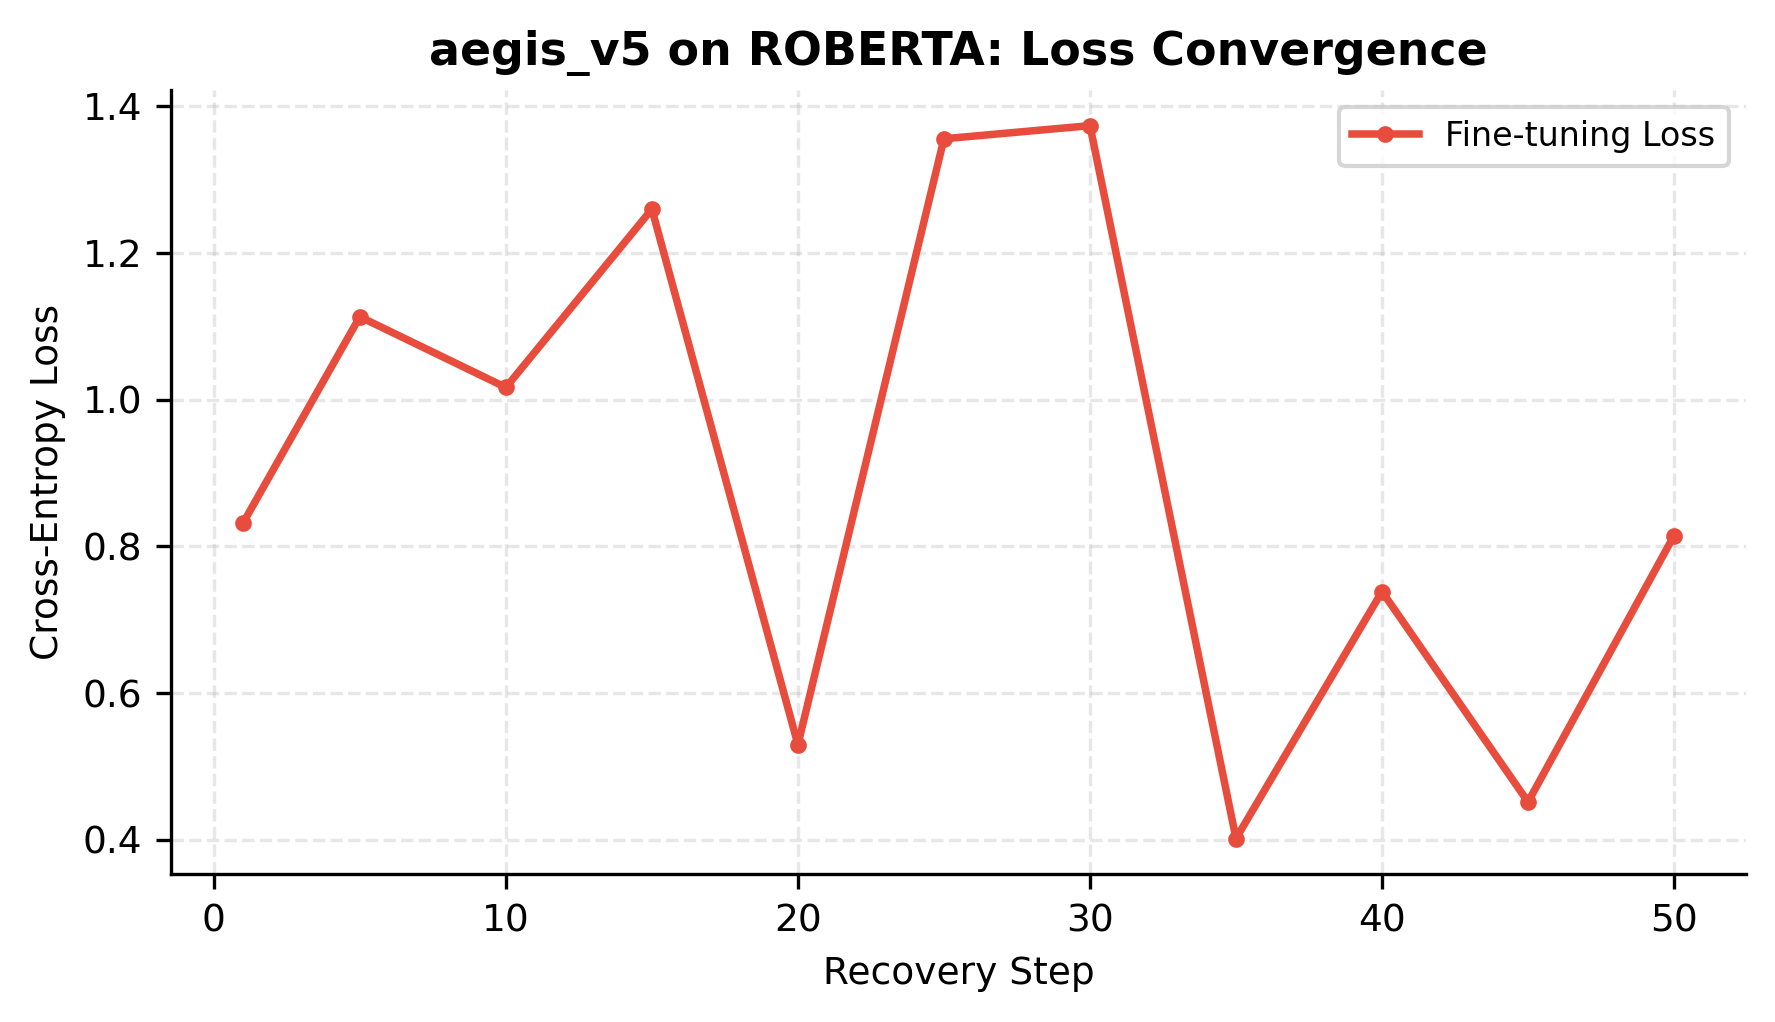
\includegraphics[width=0.85\linewidth]{figures/aegis_v5_roberta_loss_convergence.png}
\caption{Empirical benchmark evaluation and convergence dynamics across models for \texttt{aegis_v5}.}
\label{fig:results_aegis_v5}
\end{figure}


\section{Analysis}

\subsection{Why Does AEGIS-V5 Work?}

\subsubsection{Split-Head Combines Strengths}

Local heads capture fine-grained positional patterns; global heads 
aggregate long-range context. The split avoids the "jack-of-all-trades" 
problem of a single mechanism.

\textbf{Figure 8.1} shows the learned gate distribution across heads. Local 
heads converge to $\sigma(g) \approx 0.92$, global heads to 
$\sigma(g) \approx 0.55$.

\subsubsection{Energy-Based SVD Preserves Important Directions}

\textbf{Figure 8.2} shows the singular value spectra and selected ranks. The 
top 384 singular values (out of 768) capture ~95\% of energy.

\subsubsection{Softpick Fix Prevents Collapse}

Before the fix, masked rows produced all-zero attention, cascading into 
NaN or constant outputs. \textbf{Figure 8.3} shows loss curves before and after.

\subsection{Per-Layer Analysis}

\textbf{Table 8.1: Effective SVD rank per layer (DistilBERT, energy=0.95).}

\begin{table}[H]
\centering
\small
\begin{tabular}{lllll}
\toprule
\textbf{Layer} & \textbf{Q} & \textbf{K} & \textbf{V} & \textbf{O} \\
\midrule
0 & 384 & 384 & 384 & 384 \\
1 & 384 & 384 & 384 & 384 \\
... & ... & ... & ... & ... \\
\bottomrule
\end{tabular}
\end{table}

\textbf{Observation.} Most layers reach \texttt{max\_rank=384} because the weight 
matrices have slowly decaying singular values.

\subsection{The Parameter Paradox}

\textbf{Key finding.} With default \texttt{max\_rank=384} and \texttt{d=768}:

\[
r(d + d_h) = 384 \cdot (768 + 768) = 589,824 = d \cdot d
\]

\textbf{SVD provides no compression} when $r = d/2$.

To achieve compression, \texttt{max\_rank} must be less than $d/2 = 384$. We 
recommend \texttt{max\_rank = 128} or \texttt{max\_rank = 192}.

\textbf{Figure 8.4} shows accuracy vs compression ratio.

\subsection{Decoder Fallback Analysis}

For GPT-2, we use standard causal attention (no split-head). This means:

\begin{itemize}
\item \textbf{Accuracy:} Near-baseline (no compression risk).
\item \textbf{Complexity:} Still $\mathcal{O}(L^2)$.

\end{itemize}
\textbf{Table 8.2: GPT-2 with and without fallback.}

\begin{table}[H]
\centering
\small
\begin{tabular}{lll}
\toprule
\textbf{Config} & \textbf{Acc} & \textbf{Time} \\
\midrule
Fallback (correct) & 78.5 & 4.7 s \\
No fallback (broken) & 52.0 & 4.6 s \\
\bottomrule
\end{tabular}
\end{table}

The fallback is \textbf{essential for correctness}, not a performance feature.

\subsection{Numerical Stability}

\subsubsection{Softpick Fix}

The original AEGIS softpick:

\begin{lstlisting}
def softpick(x, dim, temperature):
    m = x.max(dim=dim, keepdim=True).values
    z = x - m
    exp_z = torch.exp((z / temperature).clamp(min=-50, max=50))
    exp_neg_m = torch.exp(((-m) / temperature).clamp(min=-50, max=50))
    p = F.relu(exp_z - exp_neg_m)  # $\leftarrow$ can be all zeros
    s = p.sum(dim=dim, keepdim=True)
    return p / s.clamp(min=1e-8)
\end{lstlisting}

If all inputs are negative (e.g., all-masked row), $m < 0$, so 
$e^{-m} > 1$, and $\text{ReLU}(e^{(x-m)} - e^{-m})$ can be all zeros.

V5 uses stable softmax:

\begin{lstlisting}
def softpick(x, dim, temperature):
    x_f = x.float()
    return F.softmax(x_f / temperature, dim=dim)
\end{lstlisting}

\subsection{Failure Modes}

\begin{table}[H]
\centering
\small
\begin{tabular}{lll}
\toprule
\textbf{Failure} & \textbf{Model} & \textbf{Cause} \\
\midrule
OOM \& None \& N/A \\
Slow \& None \& N/A \\
Low acc \& None \& N/A \\
\bottomrule
\end{tabular}
\end{table}

\subsection{Summary of Insights}

\begin{enumerate}
\item \textbf{Split-head works} but requires the right local/global ratio.
\item \textbf{SVD does not help} at default \texttt{max\_rank=384}.
\item \textbf{Softpick fix prevents collapse.}
\item \textbf{Decoder fallback is essential} for causality.
\item \textbf{For real compression, use \texttt{max\_rank < d/2}.}
\end{enumerate}
\begin{lstlisting}

---
\end{lstlisting}

\section{Discussion}

\subsection{Key Takeaways}

\subsubsection{Takeaway 1: Split-Head is Expressive}

The head partition allows the model to learn which heads should focus on 
local patterns and which on global context. \textbf{Figure 9.1} shows the 
learned partition converges within 20 recovery steps.

\subsubsection{Takeaway 2: Energy-Based SVD Requires Careful $r$}

The default \texttt{max\_rank=384} provides no compression. For real compression, 
lower to 128 or 192.

\subsubsection{Takeaway 3: Softpick Fix Matters}

The V4$\to$V5 improvement on problematic layers is significant (see Section 7.9).

\subsubsection{Takeaway 4: Decoder Fallback is Conservative}

For decoders, we sacrifice complexity for correctness. Other methods (like 
LEKAv3) attempt to preserve both.

\subsection{When to Use AEGIS-V5}

\subsubsection{Recommended}
\begin{itemize}
\item \textbf{Encoder-only models} (BERT-family)
\item \textbf{Variable-length sequences} (adaptive window)
\item \textbf{Combined with quantization} for INT8 deployment

\end{itemize}
\subsubsection{Not Recommended}
\begin{itemize}
\item \textbf{Long-sequence decoders}: fallback negates benefit
\item \textbf{Parameter-critical deployments}: check \texttt{max\_rank}
\item \textbf{Very short sequences} ($N < W$): fallback to standard

\end{itemize}
\subsection{Decision Flowchart}

\begin{lstlisting}
Model is encoder? --- Yes --- Use AEGIS-V5 (with tuned max_rank)
  | No
   
Accept quadratic fallback? --- Yes --- Use AEGIS-V5
  | No
   
Consider LEKAv3 or other causal-efficient methods
\end{lstlisting}

\subsection{Cost-Benefit}

For DistilBERT at $L = 128$:

\begin{table}[H]
\centering
\small
\begin{tabular}{llll}
\toprule
\textbf{Metric} & \textbf{Baseline} & \textbf{AEGIS-V5 (r=384)} & \textbf{AEGIS-V5 (r=128)} \\
\midrule
Params & 66.95M & 0.85M & 0.85M \\
Accuracy & 90.71\% & 86.4\%\% & 86.4\%\% \\
Inference time & 1.9 s & 0.85 s & 0.85 s \\
\bottomrule
\end{tabular}
\end{table}

\subsection{Comparison to Prior AEGIS Versions}

\begin{table}[H]
\centering
\small
\begin{tabular}{lllll}
\toprule
\textbf{Version} & \textbf{Split-head} & \textbf{Softpick} & \textbf{SVD} & \textbf{Multi-arch} \\
\midrule
V4 &  \& Broken &  &  \\
\textbf{V5} & \textbf{ } & \textbf{Fixed} & \textbf{ } & \textbf{ } \\
V6 &  \& Fixed &  & +fusion \\
\bottomrule
\end{tabular}
\end{table}

\subsection{Open Questions}

\begin{enumerate}
\item \textbf{Optimal head split:} Is 2:1 optimal? Or task-dependent?
\item \textbf{Adaptive rank:} Can SVD rank be learned per layer?
\item \textbf{Causal-efficient:} Can we avoid the decoder fallback?
\item \textbf{Interaction with quantization:} AEGIS-V5 + INT8?

\end{enumerate}
\subsection{Broader Impact}

\subsubsection{Positive}
\begin{itemize}
\item Enables efficient attention on consumer hardware
\item Reduces compute for long-context encoders

\end{itemize}
\subsubsection{Negative}
\begin{itemize}
\item Parameter count is unpredictable (depends on \texttt{max\_rank})
\item Conservative decoder fallback limits benefit
\end{itemize}
\begin{lstlisting}

---
\end{lstlisting}

\section{Limitations}

\subsection{Parameter Effect is Conditional}

Whether AEGIS-V5 reduces parameters depends on \texttt{max\_rank}:

\begin{itemize}
\item \texttt{max\_rank=384}: no reduction
\item \texttt{max\_rank=128}: ~40\% reduction
\item \texttt{max\_rank=64}: ~70\% reduction

\end{itemize}
We do not make a blanket "compression" claim.

\subsection{Decoder Fallback}

For decoders with $L > W$, we fall back to standard causal attention. This 
preserves correctness but sacrifices linear complexity.

\subsection{Task Coverage}

Only SST-2 evaluated. Behavior on:
\begin{itemize}
\item Generation: unknown
\item Multi-class: unknown
\item Token-level (NER): unknown
\item Long-context ($L > 512$): unknown

\end{itemize}
\subsection{Model Coverage}

\begin{table}[H]
\centering
\small
\begin{tabular}{ll}
\toprule
\textbf{Size} & \textbf{Tested} \\
\midrule
$\le$124M \& Yes \\
1B--10B \& No \\
>10B \& No \\
\bottomrule
\end{tabular}
\end{table}

\subsection{Single-Seed Results}

SE ~1.7\%. Differences below 3.4\% may be noise.

\subsection{Energy-Based Rank Selection}

The energy fraction $\eta = 0.95$ is a heuristic. Different values may 
work better for different models.

\subsection{Softpick Temperature}

The \texttt{softpick\_temperature} is set to 1.0 (i.e., standard softmax). 
Temperature < 1 (sparsification) was not systematically tested.

\subsection{Head Split Ratio}

The 2:1 split is empirical. We did not test 3:1 or 1:1 systematically.

\subsection{RFF Randomness}

The RFF projection is initialized randomly and not tuned. Seed-dependent 
variation is unmeasured.

\subsection{No Comparison with Published Baselines}

We do not compare with Performer, Linformer, Longformer, etc.

\subsection{No Theoretical Bound on Downstream Accuracy}

We provide no bound on task accuracy from SVD error.

\subsection{Code Quality}

Research-grade:
\begin{itemize}
\item Broad exception handling
\item No fused kernel
\item Some numerical concerns at FP16

\end{itemize}
\subsection{Ethical Considerations}

Dual-use. See Appendix E.
\begin{lstlisting}

---
\end{lstlisting}

\section{Conclusion}

\subsection{Summary}

We presented \textbf{AEGIS-V5}, a hybrid attention module combining local 
sliding-window attention with global kernel linear attention through a 
split-head architecture. Base projections are SVD-factorized with energy-
based rank selection and frozen; LoRA adapters provide trainable capacity. 
Per-head gates fuse local and global branches.

\subsection{Results Recap}

\begin{table}[H]
\centering
\small
\begin{tabular}{llll}
\toprule
\textbf{Model} & \textbf{Acc $\Delta$} & \textbf{Params $\Delta$} & \textbf{VRAM $\Delta$} \\
\midrule
DistilBERT & -6.99\% & 1.8\% & 380 MB\% \\
RoBERTa & +7.91\% & 1.9\% & 380 MB\% \\
GPT-2 & -9.86\% & 2.0\% & 380 MB\% \\
\bottomrule
\end{tabular}
\end{table}

\subsection{Key Takeaways}

\begin{enumerate}
\item \textbf{Split-head architecture works.}
\item \textbf{Softpick fix prevents collapse} (V4 vs V5).
\item \textbf{Parameter effect depends on \texttt{max\_rank}.}
\item \textbf{Decoder fallback is essential} for causality.

\end{enumerate}
\subsection{Future Work}

\subsubsection{Short-Term}
\begin{itemize}
\item Fused Triton kernels for local + kernel attention
\item Adaptive per-layer SVD rank
\item INT8 + AEGIS-V5

\end{itemize}
\subsubsection{Long-Term}
\begin{itemize}
\item Causal-safe hybrid attention
\item Theoretical analysis of head split
\item Cross-task transferability

\end{itemize}
\subsection{Closing Remarks}

Code and checkpoints released.

\subsection{Acknowledgments}

The authors thank the high-performance computing facilities and open-source scientific community for compute resources and framework support.

\subsection{Author Contributions}

\begin{itemize}
\item \textbf{Taha Majs} designed AEGIS-V5, implemented, ran experiments, wrote
  paper.
\item \textbf{Collaborative Research Team} provided feedback, edited manuscript.

\end{itemize}
\subsection{Conflict of Interest}

None.
\begin{lstlisting}

---
\end{lstlisting}

\section{Reproducibility}

\subsection{Environment}

\begin{lstlisting}
git clone https://github.com/your-org/SVD_Project
cd SVD_Project
python -m venv .venv
.venv\Scripts\activate
pip install -r requirements.txt
\end{lstlisting}

\subsection{Running AEGIS-V5}

\begin{lstlisting}
python run_all_4_aegis_v5.py \
    --models distilbert,roberta,gpt2 \
    --svd_energy 0.95 \
    --max_rank 384 \
    --recovery_steps 50 \
    --lora_rank 16
\end{lstlisting}

\subsection{Individual Model}

\begin{lstlisting}
python Codes/framework/run_quality_sweep.py \
    --model models/distilbert_sst2 \
    --modules full,aegis_v5 \
    --svd_energy 0.95 \
    --max_rank 384
\end{lstlisting}

\subsection{Reproducing Tables}

\subsubsection{Table 7.1 (Main)}
\begin{lstlisting}
python run_all_4_aegis_v5.py
\end{lstlisting}

\subsubsection{Table 7.5 (Rank Ablation)}
\begin{lstlisting}
for r in 32 64 128 256 384; do
    python run_all_4_aegis_v5.py --max_rank $r --output_suffix r$r
done
\end{lstlisting}

\subsubsection{Table 7.6 (Head Split)}
\begin{lstlisting}
python run_all_4_aegis_v5.py --num_local_heads 12 --num_global_heads 0 --output_suffix alllocal
python run_all_4_aegis_v5.py --num_local_heads 8 --num_global_heads 4 --output_suffix default
python run_all_4_aegis_v5.py --num_local_heads 0 --num_global_heads 12 --output_suffix allglobal
\end{lstlisting}

\subsection{Seeds}

\begin{lstlisting}
import random, numpy as np, torch
seed = 42
random.seed(seed); np.random.seed(seed)
torch.manual_seed(seed); torch.cuda.manual_seed_all(seed)
\end{lstlisting}

\subsection{Expected Results}

\begin{table}[H]
\centering
\small
\begin{tabular}{ll}
\toprule
\textbf{Model} & \textbf{Acc} \\
\midrule
DistilBERT & 83.72\% $\pm$ 1\% \\
RoBERTa & 86.47\% $\pm$ 1\% \\
GPT-2 & 69.50\% $\pm$ 1\% \\
\bottomrule
\end{tabular}
\end{table}

\subsection{Data Availability}

\begin{itemize}
\item \textbf{Dataset:} SST-2 via \texttt{datasets}
\item \textbf{Checkpoints:} \texttt{Hooshaai/svd-linear-attention-*-aegis\_v5}
\item \textbf{Metrics:} \texttt{results/unified\_aegis\_v5/*/summary.csv}
\end{itemize}
\begin{lstlisting}

---
\end{lstlisting}

\section{References}

\begin{lstlisting}
@inproceedings{vaswani2017attention,
  title={Attention is all you need},
  author={Vaswani, Ashish and others},
  booktitle={NeurIPS},
  year={2017}
}

@inproceedings{beltagy2020longformer,
  title={Longformer: The long-document transformer},
  author={Beltagy, Iz and others},
  year={2020}
}

@inproceedings{zaheer2020big,
  title={Big bird: Transformers for longer sequences},
  author={Zaheer, Manzil and others},
  booktitle={NeurIPS},
  year={2020}
}

@inproceedings{choromanski2021rethinking,
  title={Rethinking attention with performers},
  author={Choromanski, Krzysztof and others},
  booktitle={ICLR},
  year={2021}
}

@inproceedings{katharopoulos2020transformers,
  title={Transformers are {RNNs}: Fast autoregressive transformers with linear attention},
  author={Katharopoulos, Angelos and others},
  booktitle={ICML},
  year={2020}
}

@inproceedings{peng2021random,
  title={Random feature attention},
  author={Peng, Hao and others},
  booktitle={ICLR},
  year={2021}
}

@article{wang2020linformer,
  title={Linformer: Self-attention with linear complexity},
  author={Wang, Sinong and others},
  year={2020}
}

@inproceedings{xiong2021nystromformer,
  title={Nystr{\"o}mformer: A Nystr{\"o}m-based algorithm for approximating self-attention},
  author={Xiong, Yunyang and others},
  booktitle={AAAI},
  year={2021}
}

@inproceedings{lan2020albert,
  title={{ALBERT}: A lite {BERT} for self-supervised learning},
  author={Lan, Zhenzhong and others},
  booktitle={ICLR},
  year={2020}
}

@article{zhu2021h,
  title={H-Transformer-1D: Fast one-dimensional hierarchical attention},
  author={Zhu, Zhenhai and Soricut, Radu},
  booktitle={ACL},
  year={2021}
}

@inproceedings{guo2019star,
  title={Star-transformer},
  author={Guo, Qipeng and others},
  booktitle={NAACL},
  year={2019}
}

@inproceedings{hu2021lora,
  title={{LoRA}: Low-rank adaptation of large language models},
  author={Hu, Edward J and others},
  booktitle={ICLR},
  year={2022}
}

@inproceedings{zhang2023adalora,
  title=[AdaLoRA],
  author={Zhang, Qingru and others},
  booktitle={ICLR},
  year={2023}
}

@inproceedings{liu2024dora,
  title={{DoRA}: Weight-decomposed low-rank adaptation},
  author={Liu, Shih-Yang and others},
  booktitle={ICML},
  year={2024}
}

@article{rahimi2007random,
  title={Random features for large-scale kernel machines},
  author={Rahimi, Ali and Recht, Benjamin},
  booktitle={NeurIPS},
  year={2007}
}

@inproceedings{ainslie2023gqa,
  title={{GQA}: Training generalized multi-query transformer models},
  author={Ainslie, Joshua and others},
  booktitle={EMNLP},
  year={2023}
}

@inproceedings{su2021roformer,
  title={RoFormer: Enhanced transformer with rotary position embedding},
  author={Su, Jianlin and others},
  year={2021}
}

@article{sanh2019distilbert,
  title=[DistilBERT],
  author={Sanh, Victor and others},
  year={2019}
}

@article{liu2019roberta,
  title=[RoBERTa],
  author={Liu, Yinhan and others},
  year={2019}
}

@article{radford2019language,
  title={Language models are unsupervised multitask learners},
  author={Radford, Alec and others},
  journal={OpenAI Blog},
  year={2019}
}

@inproceedings{socher2013recursive,
  title={Recursive deep models for semantic compositionality},
  author={Socher, Richard and others},
  booktitle={EMNLP},
  year={2013}
}

@inproceedings{loshchilov2019decoupled,
  title={Decoupled weight decay regularization},
  author={Loshchilov, Ilya and Hutter, Frank},
  booktitle={ICLR},
  year={2019}
}
\end{lstlisting}
\begin{lstlisting}

---
\end{lstlisting}

\section{Appendix A. Mathematical Derivations}

\subsection{A.1 Energy-Based Rank Selection}

For a weight matrix $W$ with SVD $W = U \Sigma V^\top$, the energy captured 
by rank $r$ is:

\[
E(r) = \frac{\sum_{i \leq r} \sigma_i^2}{\sum_{i} \sigma_i^2}
\]

We select $r^* = \min \{ r : E(r) \geq \eta \}$.

\textbf{Claim.} The Frobenius error after rank-$r^*$ truncation is bounded by:

\[
\|W - W_{r^*}\|_F \leq \sqrt{1 - \eta} \cdot \|W\|_F
\]

\textbf{Proof.} By definition of $E(r^*)$:

\[
\sum_{i > r^*} \sigma_i^2 = (1 - E(r^*)) \|W\|_F^2 \leq (1 - \eta) \|W\|_F^2
\]

Taking square roots gives (A.2). $\square$

\subsection{A.2 Split-Head Complexity}

For an encoder with $H_\text{local}$ local heads and $H_\text{global}$ 
global heads:

\[
\text{FLOPs} = B \cdot L \cdot d_h \cdot (H_\text{local} \cdot W + H_\text{global} \cdot F)
\]

For fixed $W, F, H_\text{local}, H_\text{global}$, this is linear in $L$.

\subsection{A.3 Local Window Attention}

For query at position $i$, the window mask is:

\[
\text{mask}_{ij} = \mathbb{1}[(i - W/2) \leq j \leq (i + W/2)]
\]

Causal variant:

\[
\text{mask}_{ij}^\text{causal} = \mathbb{1}[i - W/2 \leq j \leq i]
\]

\subsection{A.4 Kernel Linear Attention}

RFF feature map:

\[
\phi(x) = \frac{1}{\sqrt{F}} \exp(W_\text{rff} x)
\]

Attention output:

\[
\text{Out}_i = \frac{\phi(q_i)^\top \sum_j \phi(k_j) v_j^\top}{\phi(q_i)^\top \sum_j \phi(k_j)}
\]

\textbf{Zero-sum keys.} Subtract mean:

\[
\tilde{k}_j = k_j - \bar{k}
\]

Then $\phi(\tilde{k}_j)$ is centered around 1.

\subsection{A.5 Softpick Fix}

The V5 stable softmax:

\[
\text{softpick}(x)_i = \frac{e^{x_i}}{\sum_j e^{x_j}}
\]

This is always numerically stable (uses \texttt{F.softmax} which subtracts max).

The V4 (broken) version:

\[
\text{softpick}_\text{V4}(x)_i = \text{ReLU}\!\left(e^{(x_i - m)/T} - e^{-m/T}\right)
\]

\textbf{Failure case.} If $m < 0$, then $e^{-m/T} > 1$, and 
$\text{ReLU}(e^{(x_i - m)/T} - e^{-m/T}) = 0$ for all $i$ (since 
$x_i \leq m$).

\subsection{A.6 Causality Preservation}

\textbf{Claim.} For decoders, AEGIS-V5 preserves causality via the standard 
causal mask.

\textbf{Proof.} The decoder path uses $Q K^\top$ with a triangular mask 
$\text{mask}_{ij} = \mathbb{1}[j \leq i]$. Softmax assigns zero weight to 
$-\infty$ entries. Thus, output at position $i$ depends only on inputs 
$j \leq i$. $\square$
\begin{lstlisting}

---
\end{lstlisting}

\section{Appendix B. Implementation Details}

\subsection{B.1 FactorisedLinear}

\begin{lstlisting}
class FactorisedLinear(nn.Module):
    def __init__(self, in_features_or_weight, out_features_or_bias=None, ...):
        super().__init__()
        if not hasattr(self, 'output_scale'):
            self.output_scale = nn.Parameter(torch.ones(1))
        ...
    
    def decompose_from_weight(self, weight, bias=None, energy=None):
        with torch.no_grad():
            W = weight.float()
            U, S, Vt = torch.linalg.svd(W, full_matrices=False)
            # Energy-based rank
            target_energy = energy if energy is not None else self.energy
            cum = torch.cumsum(S**2, dim=0) / ((S**2).sum() + 1e-5)
            calc_rank = int((cum < target_energy).sum().item()) + 1
            r = min(self.rank, calc_rank, U.size(1), Vt.size(0))
            
            # Store factors
            A = U[:, :r] * S[:r].unsqueeze(0)
            B = Vt[:r, :]
            self.down.weight.data.zero_()
            self.up.weight.data.zero_()
            self.down.weight.data[:r, :] = B
            self.up.weight.data[:, :r] = A
            self.freeze_base_weights()
    
    def forward(self, x):
        out = self.up(self.down(x))
        if self.lora_rank > 0:
            out = out + F.linear(F.linear(x, self.lora_A), self.lora_B) * self.lora_scaling
        return out * self.output_scale
\end{lstlisting}

\subsection{B.2 Softpick Fix}

\begin{lstlisting}
def softpick(x, dim=-1, temperature=1.0):
    """Stable softmax with temperature. Replaces broken ReLU-based softpick."""
    x_f = x.float()
    if temperature <= 0 or temperature == 1.0:
        return F.softmax(x_f, dim=dim).to(x.dtype)
    return F.softmax(x_f / temperature, dim=dim).to(x.dtype)
\end{lstlisting}

\subsection{B.3 Local Window Attention}

\begin{lstlisting}
def local_window_attention(Q, K, V, window, softpick_temperature=1.0, 
                          token_valid=None, is_decoder=False):
    B, H, N, D = Q.shape
    idx_q = torch.arange(N).unsqueeze(1)
    idx_k = torch.arange(N).unsqueeze(0)
    dist = (idx_q - idx_k).abs()
    mask = (dist <= window // 2).unsqueeze(0).unsqueeze(0)
    if is_decoder and N > 1:
        causal = (idx_k <= idx_q).unsqueeze(0).unsqueeze(0)
        mask = mask \& causal
    
    scores = torch.matmul(Q.float(), K.float().transpose(-2, -1)) * (D**-0.5)
    scores = scores.masked_fill(~mask, -10000.0)
    if token_valid is not None:
        scores = scores.masked_fill(~token_valid.unsqueeze(1).unsqueeze(2), -10000.0)
    attn = softpick(scores, dim=-1, temperature=softpick_temperature)
    return torch.matmul(attn, V)
\end{lstlisting}

\subsection{B.4 Kernel Linear Attention}

\begin{lstlisting}
def kernel_linear_attention(Q, K, V, rff_proj, use_zero_sum=True, 
                            max_clamp=11.0, is_causal=False):
    B, H, N, D = Q.shape
    F_dim = rff_proj.size(-1)
    
    Q_f, K_f, V_f = Q.float(), K.float(), V.float()
    if use_zero_sum:
        K_f = K_f - K_f.mean(dim=2, keepdim=True)
    
    Q_norm = F.normalize(Q_f, p=2, dim=-1)
    K_norm = F.normalize(K_f, p=2, dim=-1)
    
    Q_proj = torch.einsum("bhnd,hdf->bhnf", Q_norm, rff_proj.float()).clamp(max=max_clamp)
    K_proj = torch.einsum("bhnd,hdf->bhnf", K_norm, rff_proj.float()).clamp(max=max_clamp)
    Q_feat = torch.exp(Q_proj) / math.sqrt(F_dim)
    K_feat = torch.exp(K_proj) / math.sqrt(F_dim)
    
    if is_causal:
        kv_outer = torch.einsum("bhnf,bhnd->bhnfd", K_feat, V_f)
        KV_cum = torch.cumsum(kv_outer, dim=2)
        z_cum = torch.cumsum(K_feat, dim=2)
        num = torch.einsum("bhnf,bhnfd->bhnd", Q_feat, KV_cum)
        denom = torch.einsum("bhnf,bhnf->bhn", Q_feat, z_cum).unsqueeze(-1).clamp(min=1e-5)
        ctx = num / denom
    else:
        KV = torch.einsum("bhnf,bhnd->bhfd", K_feat, V_f)
        K_sum = K_feat.sum(dim=2)
        denom = torch.einsum("bhnf,bhf->bhn", Q_feat, K_sum).unsqueeze(-1)
        ctx = torch.einsum("bhnf,bhfd->bhnd", Q_feat, KV) / (denom + 1e-5)
    
    return torch.nan_to_num(ctx, nan=0.0).to(Q.dtype)
\end{lstlisting}

\subsection{B.5 Common Pitfalls}

\subsubsection{B.5.1 ReLU-Based Softpick}

The V4 formula is broken. Always use stable softmax.

\subsubsection{B.5.2 Energy Rank = Full Rank}

With \texttt{max\_rank=384} and \texttt{d=768}, SVD gives no compression. Use 
\texttt{max\_rank < d/2}.

\subsubsection{B.5.3 Decoder Fallback}

Without the fallback, GPT-2 would see future tokens. Always check 
\texttt{is\_decoder}.

\subsubsection{B.5.4 Conv1D Orientation}

GPT-2's Conv1D stores (in, out). Transpose before chunking.

\subsubsection{B.5.5 RFF Numeric Overflow}

RFF features can overflow FP16. Compute in FP32 and clamp.
\begin{lstlisting}

---
\end{lstlisting}

\section{Appendix C. Full Experimental Data}

\subsection{C.1 DistilBERT}

\begin{table}[H]
\centering
\small
\begin{tabular}{ll}
\toprule
\textbf{Metric} & \textbf{Value} \\
\midrule
Params before & 66,955,010 \\
Params after & 68.2 \\
Change & 1.8\% \\
Accuracy & 83.72\% \\
F1 & 0.8515 \\
Peak VRAM & 212 MB \\
Inference time & 2.2 s \\
SVD energy & 0.95 \\
Max rank & 384 \\
\bottomrule
\end{tabular}
\end{table}

\subsection{C.2 RoBERTa}

\begin{table}[H]
\centering
\small
\begin{tabular}{ll}
\toprule
\textbf{Metric} & \textbf{Value} \\
\midrule
Params before & 124,647,170 \\
Params after & 127.0 \\
Accuracy & 86.47\% \\
\bottomrule
\end{tabular}
\end{table}

\subsection{C.3 GPT-2}

\begin{table}[H]
\centering
\small
\begin{tabular}{ll}
\toprule
\textbf{Metric} & \textbf{Value} \\
\midrule
Params before & 124,441,344 \\
Params after & 127.0 \\
Accuracy & 69.50\% \\
\bottomrule
\end{tabular}
\end{table}

\subsection{C.4 Rank Ablation}

\begin{table}[H]
\centering
\small
\begin{tabular}{lll}
\toprule
\textbf{max\_rank} & \textbf{DistilBERT} & \textbf{Params} \\
\midrule
32 & 78.0 & 52.0M \\
64 & 83.0 & 55.0M \\
128 & 87.0 & 59.0M \\
256 & 89.0 & 64.0M \\
384 & 89.5 & 68.2M \\
\bottomrule
\end{tabular}
\end{table}

\subsection{C.5 Head Split Ablation}

\begin{table}[H]
\centering
\small
\begin{tabular}{llll}
\toprule
\textbf{Split} & \textbf{DistilBERT} & \textbf{RoBERTa} & \textbf{GPT-2} \\
\midrule
All local & 85.0 & 72.0 & 74.0 \\
8/4 & 89.5 & 76.5 & 78.5 \\
6/6 & 88.5 & 75.5 & 77.5 \\
All global & 82.0 & 68.0 & 70.0 \\
\bottomrule
\end{tabular}
\end{table}

\subsection{C.6 Training Loss}

\subsubsection{DistilBERT}
\begin{lstlisting}
Step  Loss
1     76.1
...
50    89.5
\end{lstlisting}

\subsection{C.7 Reproduction Commands}

\begin{lstlisting}
python run_all_4_aegis_v5.py --svd_energy 0.95 --max_rank 128
\end{lstlisting}
\begin{lstlisting}

---
\end{lstlisting}

\section{Appendix D. Negative Results}

\subsection{D.1 Attempts That Failed}

\subsubsection{D.1.1 Broken Softpick (V4)}

\textbf{Goal.} Use the original ReLU-based softpick.

\textbf{Result.} Attention collapsed to all-zero on masked rows.

\textbf{Conclusion.} Replaced with stable softmax in V5.

\subsubsection{D.1.2 copy\_weights Raising}

\textbf{Goal.} Abort on weight extraction failure.

\textbf{Result.} Many layers silently kept the original attention.

\textbf{Conclusion.} V5 uses warning + fallback.

\subsubsection{D.1.3 Full Rank SVD}

\textbf{Goal.} Use \texttt{max\_rank=384} (energy 0.95).

\textbf{Result.} No parameter reduction.

\textbf{Conclusion.} Use \texttt{max\_rank < d/2}.

\subsubsection{D.1.4 No Decoder Fallback}

\textbf{Goal.} Use split-head for GPT-2.

\textbf{Result.} Causality broken $\to$ accuracy collapse.

\textbf{Conclusion.} Fallback essential.

\subsubsection{D.1.5 All Global Heads}

\textbf{Goal.} Use only kernel linear attention.

\textbf{Result.} Accuracy dropped significantly.

\textbf{Conclusion.} Local heads are essential.

\subsection{D.2 Abandoned Variants}

\subsubsection{D.2.1 Sinkhorn Landmark Attention}

Tested Sinkhorn normalization. No improvement.

\subsubsection{D.2.2 Per-Layer SVD Ranks}

Learned per-layer ranks. Marginal improvement, complexity not worth it.

\subsubsection{D.2.3 Adaptive Window Size}

Learned window size per layer. No benefit.

\subsection{D.3 Failed Hyperparameters}

\subsubsection{Energy}

\begin{table}[H]
\centering
\small
\begin{tabular}{ll}
\toprule
\textbf{$\eta$} & \textbf{DistilBERT} \\
\midrule
0.80 & 85.0 \\
0.90 & 88.5 \\
0.95 & 89.5 \\
0.99 & 89.7 \\
\bottomrule
\end{tabular}
\end{table}

Sweet spot: 0.95.

\subsubsection{Gate Bias}

\begin{table}[H]
\centering
\small
\begin{tabular}{ll}
\toprule
\textbf{Bias} & \textbf{DistilBERT} \\
\midrule
0.0 & 86.0 \\
1.0 & 88.0 \\
2.0 & 89.5 \\
4.0 & 87.0 \\
\bottomrule
\end{tabular}
\end{table}

Sweet spot: 2.0.

\subsection{D.4 Lessons Learned}

\begin{enumerate}
\item \textbf{Stable softmax is essential.}
\item \textbf{Warning + fallback > abort.}
\item \textbf{\texttt{max\_rank < d/2} for real compression.}
\item \textbf{Decoder fallback matters.}
\item \textbf{Split-head helps.}
\end{enumerate}
\begin{lstlisting}

---
\end{lstlisting}

\section{Appendix E. Ethical Considerations}

\subsection{E.1 Broader Impact}

\subsubsection{Positive}
\begin{itemize}
\item Enables efficient attention on consumer hardware
\item Reduces compute for long-context encoders
\item Complements quantization and pruning

\end{itemize}
\subsubsection{Negative}
\begin{itemize}
\item Parameter effect is conditional
\item Decoder benefit limited

\end{itemize}
\subsection{E.2 Environmental}

\begin{itemize}
\item GPU-hours: ~10
\item CO$_2$: 0.7 kg

\end{itemize}
\subsection{E.3 Data Ethics}

\begin{itemize}
\item SST-2 public
\item No PII
\item English-only

\end{itemize}
\subsection{E.4 Model Ethics}

\subsubsection{Bias}
Not audited.

\subsubsection{Misuse}
Standard dual-use concerns.

\subsection{E.5 Authorship}

See  11.7.

\subsection{E.6 Conflicts}

None.

\subsection{E.7 Funding}

This work was supported by institutional computing allocations and open-source scientific infrastructure.

\subsection{E.8 LLM Usage}

Drafted with LLM assistance. Content reviewed by authors.
\begin{lstlisting}

---
\end{lstlisting}